\section{Synthèse du développement Java}
\label{sec:synthese_java}
En termes de temps investi, le développement Java était à peu près équivalent à l'intégration continue dans mon stage. Le travail effectué sera plus court à synthétiser cependant, en ce sens qu'il se rapproche plus à ce que j'ai pu connaître de Java au cours de ma formation.

\subsection{Rappel du contexte}
J'ai travaillé sur plusieurs projets en Java, mais il n'y en a qu'un où mon intervention n'a pas été anecdotique : un projet de gestion de tests de voiture pour un constructeur automobile. Le client avait utilisé pendant longtemps un middleware propriétaire pour la communication client/serveur, et avait décidé de changer pour ActiveMQ en même temps que de changer de prestataire pour le développement du logiciel (c'est à cette occasion qu'Alter Frame a récupéré le contrat).

La solution initiale était Notify (je n'ai pas réussi à trouver de documentation là-dessus), mais celle-ci avait déjà disparu à mon arrivée sur le projet. En revanche, ActiveMQ n'était pas encore pleinement fonctionnel, son intégration ayant entraîné des régressions et des bugs nouveaux.

Malgré cela, ce changement était utile d'une part pour l'économie du prix de la licence (Apache ActiveMQ est librement distribué sous licence Apache 2.0... sans surprise) et d'autre part pour profiter de la stabilité d'une solution plus largement adoptée et maintenue.

En plus du développement à proprement parler, j'ai au à créer un installeur pour le logiciel en question, ce qui s'est avéré beaucoup moins trivial que ce que j'avais tout d'abord anticipé.

\subsection{ActiveMQ}
L'intégration d'ActiveMQ à un projet Java est simple : un des interlocuteurs crée une connexion, un message qui doit nécessairement avoir une destination, et un producteur qui est le processus qui va se charger de l'envoi à proprement parler. Les actions sont presque identiques pour le deuxième interlocuteur, excepté que celui-ci crée un consommateur\cite{activemq_intro} (voir listing~\ref{lst:activemqex} tiré de la documentation).

L'avantage du système de queue d'ActiveMQ est que le producteur et le receveur n'ont pas besoin d'être disponibles en même temps, le \textit{broker} (le daemon qui reçoit et  transmet les messages) les garde en mémoire jusqu'à ce qu'ils soient consommés. C'est la destination qui sert à savoir qui reçoit quoi : elle correspond à une queue, quand un expéditeur renseigne cette destination un message est ajouté à la file et quand c'est un consommateur, un message est retiré de la file (c'est un modèle FIFO).

ActiveMQ propose une interface web pour visualiser le traffic géré par le \textit{broker}, les différentes queues, le nombre de producteurs/consommateurs, nombre de messages échangés, etc, à l'adresse \url{http://localhost:8161/admin/}.

\begin{minipage}{\linewidth}
	\begin{lstlisting}[language=Java, caption="Un exemple écourté d'échange de messages \textit{via} ActiveMQ", label={lst:activemqex}]
  public static class HelloWorldProducer implements Runnable {
    public void run() {
        try {
            ActiveMQConnectionFactory connectionFactory = new ActiveMQConnectionFactory("vm://localhost");

            Connection connection = connectionFactory.createConnection();
            connection.start();

            Session session = connection.createSession(false, Session.AUTO_ACKNOWLEDGE);

            Destination destination = session.createQueue("TEST.FOO");

            MessageProducer producer = session.createProducer(destination);
            producer.setDeliveryMode(DeliveryMode.NON_PERSISTENT);

            String text = "Hello world! From: " + Thread.currentThread().getName() + " : " + this.hashCode();
            TextMessage message = session.createTextMessage(text);

            producer.send(message);

            session.close();
            connection.close();
        }
        catch (Exception e) {
            System.out.println("Caught: " + e);
            e.printStackTrace();
        }
    }
}

public static class HelloWorldConsumer implements Runnable, ExceptionListener {
    public void run() {
        try {
            ActiveMQConnectionFactory connectionFactory = new ActiveMQConnectionFactory("vm://localhost");
            Connection connection = connectionFactory.createConnection();
            connection.start();
            connection.setExceptionListener(this);
            Session session = connection.createSession(false, Session.AUTO_ACKNOWLEDGE);
            Destination destination = session.createQueue("TEST.FOO");
            MessageConsumer consumer = session.createConsumer(destination);

            Message message = consumer.receive(1000);

            if (message instanceof TextMessage) {
                TextMessage textMessage = (TextMessage) message;
                String text = textMessage.getText();
                System.out.println("Received: " + text);
            } else {
                System.out.println("Received: " + message);
            }

            consumer.close();
            session.close();
            connection.close();
        } catch (Exception e) {
            System.out.println("Caught: " + e);
            e.printStackTrace();
        }
    }
\end{lstlisting}
\end{minipage}

La mécanique de départ est assez simple et c'est tout l'intérêt de cet outil ; la vraie difficulté a résidé dans la recherche de toutes les utilisations qui étaient faites de l'ancienne librairie Notify, et leur remplacement sans générer d'effet de bord ; plus facile à dire qu'à faire comme toujours quand il s'agit de refactorer du code !

Il est difficile d'isoler un exemple de code sur lequel j'ai travaillé, tant cela a été de petites retouches à différents endroits des sources, suivis de longues sessions de tests avec le chef de projet pour exposer toutes les conséquences des modifications et, s'il y en avait d'inattendues, les corriger. Voici tout de même un exemple notable : listings~\ref{lst:lock_un} et~\ref{lst:lock_deux}.

\begin{minipage}{\linewidth}
	\begin{lstlisting}[language=Java, caption="Gestion des verrous à la réception d'un message côté client", label={lst:lock_un}]
public void onMessage(Message rawMsg) {
    switch (duo.getFirst()) {
        case BDD :
            switch (duo.getSecond()) {
                case NOTIFY_LOCK :
                    CustomLogEngine.debug("NotifyConnector - srvMsgProcess : notify lock");
                    callId = msg.getNextShort();
                    sender = msg.getNextString();
                    error = msg.getNextString();
                    CacheClient.getClientForNotify().notifyLockFromServer(error, callId);
                    break;
                case NOTIFY_UNLOCK :
                    CustomLogEngine.debug("NotifyConnector - srvMsgProcess : notify lock");
                    callId = msg.getNextShort();
                    sender = msg.getNextString();
                    short callIdToUnlock = msg.getNextShort();
                    error = msg.getNextString();
                    CacheClient.getClientForNotify().notifyUnlockFromServer(error, callIdToUnlock, callId); 
                    break;

                // ...

            }
        case ALL_TYPE :
            switch (duo.getSecond()) {
                case LOCK :
                    // A chaque accès à une ressource
                    // synchronisée on reçoit la liste des lock que nous
                    // fournit le serveur
                    updateLocalLockMap(msg);
                    break;

                // ...

            }

        // ...
                
    }
}
    \end{lstlisting}
\end{minipage}

\begin{minipage}{\linewidth}
	\begin{lstlisting}[language=Java, caption="Méthode permettant de mettre à jour les ressources verrouillées", label={lst:lock_deux}]
private void updateLocalLockMap(CustomMessage msg) {
    String dest = msg.getDest();
    if (this.applicationName.equals(dest)) {
        synchronized (MainModel.getInstance().getMapLock()) {
            try {
                if (msg.hasNextData()) {
                    CustomLocker mapl = (CustomLocker) msg.getNextObject();
                    if (mapl != null) {
                        MainModel.getInstance().setMapLock(mapl.getMapLock());
                    }
                }
            } catch (Exception e) {
                CustomLogEngine.error(CustomLogEngine.getStackTrace(e));
            }
        }
    }
}
    \end{lstlisting}
\end{minipage}

Le logiciel en question gère la modification d'affaires, c'est-à-dire du récapitulatif de l'état d'un véhicule en termes de tests qui ont été effectués dessus, des résultats obtenus jusque là, etc. Tous les clients connectés à un même serveur peuvent visualiser ces affaires en même temps, mais un seul peut en modifier une à la fois pour éviter des modifications concurrentes de la base de données.

Échanger efficacement les informations sur un tel verrou, les maintenir à jour et les faire respecter, s'est avéré une tâche longue et difficile. Les listings cités plus haut représentent la partie client de ce code, que j'ai partiellement écrite : on maintient une \textit{map} de verrous qui associe à une ressource l'utilisateur qui en possède le verrou (ou ne contient pas d'entrée, si la ressource est libre). 

Quand un client essaie d'accéder à une telle ressource, on vérifie la présence de la ressource dans la \textit{map} ; si elle est présente l'utilisateur voit un message d'erreur apparaître et sinon, il ouvre la ressource et envoie simultanément un \textit{lock} au serveur qui va le diffuser à tous les utilisateurs connectés en plus de mettre à jour sa propre \textit{map} des verrous pour pouvoir la transmettre aux nouveaux utilisateurs qui se connectent. 

\subsection{Création d'un installeur}
Il ne s'agit là pas de Java mais de NSIS\cite{nsis} : un outil open source pour générer des (dés)installeurs sous Windows, indépendants du langage de l'application à installer. NSIS est également le nom du langage de script utilisé pour créer l'installeur ; complexe mais d'une grande flexibilité, il couvre un large éventail de fonctionnalités et a surtout une documentation de qualité, claire et détaillée\cite{nsis_doc}. 

Un résumé de la construction d'un script NSIS : un installeur est composé de page, ce sont les différentes fenêtres qui s'affichent au cours de l'installation. NSIS propose les plus classiques par défaut (e.g. choisir le chemin d'installation) et des pages personnalisées peuvent être créées. L'installeur affiche les pages dans l'ordre dans lequel elles sont déclarées dans le script. 

Chaque page comporte une ou plusieurs fonctions qui détaillent son fonctionnement, peuvent annuler l'affichage de la page ou empêcher l'utilisateur de passer à la suivante sous certaines conditions (e.g. \og Vous devez fermer l'application avant de la désinstaller \fg).

Enfin, des sections sont appelées pour l'installation à proprement parler des éléments. La différence avec les fonctions est que ces dernières définissent le comportement de la page d'un point de vue GUI. Les sections vont modifier le registre, copier des fichiers, créer des raccourcis, etc. La page par défaut \verb|COMPONENTS| permet à l'utilisateur de choisir les composants qu'il installe, chaque composant correspond à une section du même nom, et la page par défaut \verb|INSTFILES| installe chaque section correspondant à un composant sélectionné. 

Des exemples typiques sont proposés avec l'installation de NSIS, l'installation des composants principaux de l'application n'a donc pas demandé de grandes modifications excepté le chemin vers les différents éléments. Un composant plus intéressant est la page proposant de désinstaller une version précédente de l'application avant d'installer la version actuelle (cf. capture d'écran~\ref{nsis_unins}).

\begin{figure}
    \centering
    \caption{Écran de désinstallation}
	\label{fig:nsis_unins}
    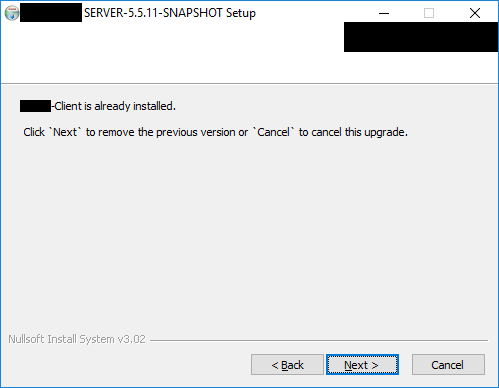
\includegraphics[width=\textwidth]{images/nsis_uninstall}
\end{figure}

Un si simple message a demandé beaucoup de travail car il fallait d'une part comprendre le fonctionnement de NSIS pour ne l'afficher que sous certaines conditions, et d'autre part se pencher sur celui de Windows pour vérifier la présence d'une installation précédente.

\begin{lstlisting}[caption="Script NSIS permettant de désinstaller puis réinstaller une application", label={lst:nsis_script}]
    Page custom checkIfAlreadyInstalled checkIfRunning
    Page custom uninstallBeforeInstall ""        
    
    Var Tmp
    Var AlreadyInstalled
    Var UninstallerPath
    
    Function checkIfAlreadyInstalled
        StrCpy $AlreadyInstalled "false"
    
        ReadRegStr $UninstallerPath HKCU \
        "Software\Microsoft\Windows\CurrentVersion\Uninstall\${setup.regKey}" \
        "UninstallString"
        StrCmp $UninstallerPath "" abort
    
        nsDialogs::Create 1018
        Pop $Tmp
    
        StrCpy $AlreadyInstalled "true"
    
        ${If} $Tmp == error
            Abort
        ${EndIf}
    
        ${NSD_CreateLabel} 0 0 100% 50% \
        "Client is already installed. $\n$\nClick `Next` to remove the \
        previous version or `Cancel` to cancel this upgrade."
        Pop $Tmp
        ${If} $Tmp == error
            Abort
        ${EndIf}
    
        nsDialogs::Show
        Goto done
    
        abort:
            Abort
        done:
    FunctionEnd
    
    Function uninstallBeforeInstall
        StrCmp $AlreadyInstalled "false" abort
        HideWindow
        ClearErrors 
        ExecWait '$UninstallerPath _?=$INSTDIR'
        BringToFront
        IfErrors no_remove_uninstaller done
        Delete $UninstallerPath
        RMDir $INSTDIR
        no_remove_uninstaller:
            Goto done
        abort:
            Abort
        done:
    FunctionEnd
    
    Function checkIfRunning
        FindProcDLL::FindProc "${exe}"
        IntCmp $R0 1 0 notRunning
            MessageBox MB_OK|MB_ICONEXCLAMATION "client is running. Please close it first" /SD IDOK
            Abort
        notRunning:
    FunctionEnd       

    Section "Uninstall"
        DeleteRegKey HKCU "Software\Microsoft\Windows\CurrentVersion\Uninstall\${setup.regKey}"
        DeleteRegKey HKCU "Software\${setup.regKey}"
    
        RMDir /r /REBOOTOK $INSTDIR
    
        Delete "$DESKTOP\${diplayName}.lnk"
    
        Delete "$SMPROGRAMS\${setup.dir}\*.*"
    
        RMDir "$SMPROGRAMS\${setup.dir}"
    SectionEnd        
\end{lstlisting}

Comme on peut le voir dans le listing~\ref{lst:nsis_script}, NSIS est un langage verbeux dans le sens où peu de choses sont gérées automatiquement à la génération de l'installeur : le script doit détailler chaque étape. Dans l'extrait présenté ici, je crée deux pages, une qui vérifie la présence d'une installation précédente, et le cas échéant qui vérifie si l'application est en cours d'utilisation, et une qui propose à l'utilisateur de désinstaller l'application. 

Aucune de ces pages ne s'affiche si l'application n'est pas déjà présente sur le système : c'est l'effet de \verb|abort| lignes 14 et 42 (bien qu'à proprement parler il s'agisse de jumps qui renvoient au véritable appel à \verb|Abort| plus loin). On utilise le registre Windows pour détecter la présence de l'application sur le système, et une librairie (\verb|FindProcDLL|) pour obtenir de Windows la liste des processus en cours d'utilisation et y chercher le nom du nôtre. 

Les variables, de la forme \verb|${nomVariable}|, qui ne sont pas définies explicitement ici sont importées du \verb|pom.xml| du projet. Expliquer chaque point du script prendrait trop de temps ici (j'ai justement écrit une documentation bien plus complète sur NSIS, en Markdown, mais celle-ci n'est disponible que sur le serveur GitLab privé d'Alter Frame), mais cet extrait donne une idée générale du langage NSIS et de ses forces et faiblesses.